% GATE: spec \S 9-B -- do not \input this file into the compiled body until
% the check below is done. Kept as a complete, ready-to-activate figure so
% activating it later is a one-line change (uncomment the \input in
% experiments.tex) once the gate clears.
\begin{figure}[t]
\centering
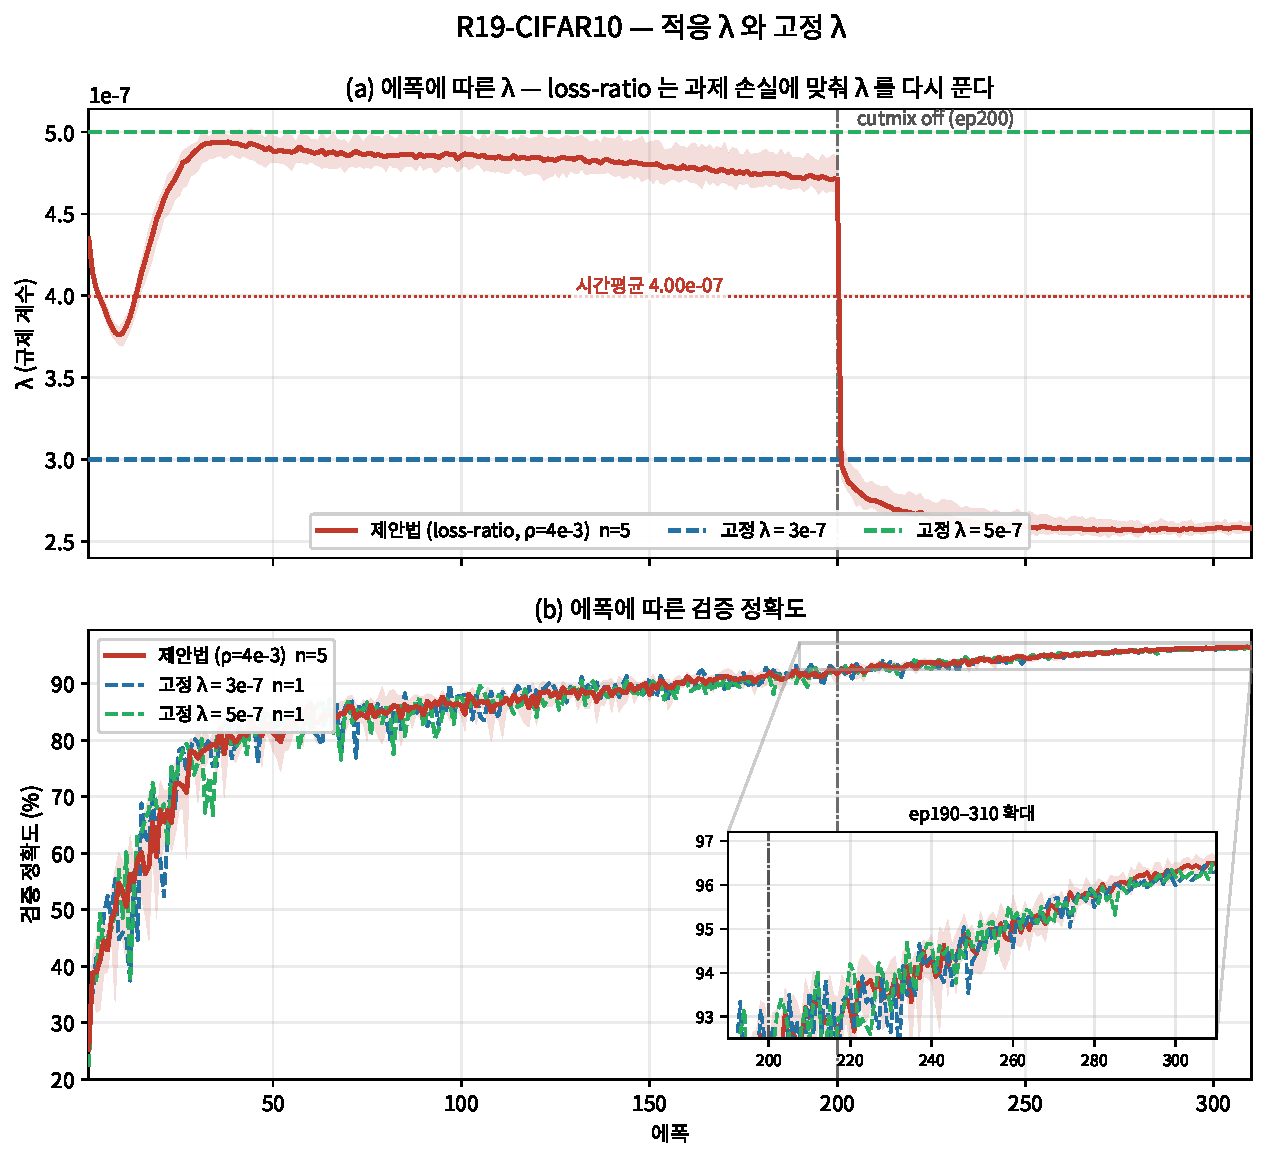
\includegraphics[width=\linewidth]{figures/f6_lambda_epoch_appendix.pdf}
\caption{GATE: spec \S 9-B -- the 44\% drop in $\lambda$ at epoch 201
coincides with CutMix switching off (\texttt{mix\_off\_iter}\,$=500{\times}200$),
but whether it also coincides with a specific point in the learning-rate
schedule has not been checked. Do not read this trajectory as
schedule-independent until that check is done; if the two coincide, the
ratio controller would be indirectly schedule-dependent, for the same
reason the \texttt{lr-linked} variant was rejected earlier (spec \S 9-B).}
\label{fig:f6_lambda}
\end{figure}
